% !TEX root = ../ausarbeitung.tex
%%% DELETE THIS LATER
%Im Hauptteil beschreiben Sie Ihre praktische Arbeit. Code gehört %normalerweise nicht in eine Ausarbeitung. Ausnahmen sind Algorithmen, %die für Sie wichtig waren (dann in möglichst übersichtlichem Pseudo-%Code). Kleine Code-Stücke können auch zur Illustration oder als Beispiel %eingebaut werden. Längere Code-Stücke können im Anhang %untergebracht werden. Sie sollten jedoch nicht den gesamten Code im %Anhang abdrucken. Ihren Code geben Sie bitte dennoch mit ab, am %besten auf einer CD.
%
%Der Detailgrad sollte so sein, dass ein Leser die gleiche Arbeit noch %einmal nachimplementieren könnte. Insbesondere sollten alle Parameter, %von denen die Funktionsweise des Systems abhängt, explizit genannt %sein. Bei der Evaluation muss bei jedem Versuch angegeben werden, mit %welchen Parametern gearbeitet wird.
\chapter{Herangehensweise}
In diesem Kapitel wird der Weg von der Konzipierung mehrerer Konzepte für das Lernspiel bis zur Implementierung des Spiels behandelt.
\section{Konzeptwahl des Spiels}
\subsection{Erste Idee Math Smashers}
Die erste Idee ein Lernspiel zu entwickeln, welches Grundschüler unterstützt die Addition über das Konzept der Partnerzahlen zu erlernen, war das bereits vorhandene Spiel \textit{Math Smashers}\cite{ludoscience}.\\
In \textit{Math Smashers} fliegen Bälle mit Zahlen herum. Als Spieler kann man eine Art Seil als Verbindung zwischen zwei Kugeln anbringen. Dieses Seil zieht sich zusammen um die Kugeln zusammenzufassen (siehe \ref{fig:mathsmashers}) und deren Zahlen zu addieren (z.B. eine Kugel mit der Zahl 18 und eine mit der Zahl 4 gibt zusammengefasst eine Kugel mit der Zahl 22). Ziel ist es alle Bälle so zu addieren, damit man eine gesuchte Zahl (z.B. 22) heraus bekommt. Dabei kann es auch vorkommen mehrmals die gesuchte Zahl zu bekommen.
\begin{figure}[htb]
	\centering
	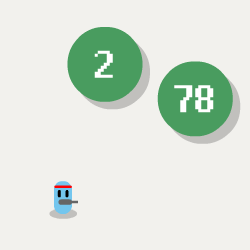
\includegraphics[width=0.3\textwidth]{MathSmasher-NotConnected}
	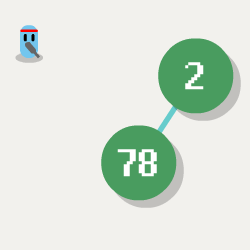
\includegraphics[width=0.3\textwidth]{MathSmasher-Connected}
	\caption{MathSmashers links zwei nicht verbundene Zahlen. Rechts beide Zahlen verbunden.\label{fig:mathsmashers}}
\end{figure}
\subsection{Weitere Ideenfindung}
Zunächst wurden weitere Ideen erarbeitet, wie das Konzept der Partnerzahlen noch in einem Spiel untergebracht werden kann. Dabei entstanden die folgenden vier Ideen.
\subsubsection{Kombination mit \qq{The Legend of Zelda}}
Diese Idee ist als Anlehnung an das Spiel \textit{The Legend of Zelda} gedacht. Kombiniert wird es mit dem bereits beschriebenen \textit{Math Smashers}. In diesem Fall werden, statt Bällen, die aus \textit{The Legend of Zelda: Majoras Mask}\cite{zelda} bekannten Schleimgegner, die Zahlen enthalten, verwendet. Ziel ist es auch hier zwei Zahlen zu einer Gesuchten zu addieren, indem Schleimgegner mit den passenden Partnerzahlen besiegt und die im Schleim liegenden Zahlen addiert.
\begin{figure}[htb]
	\centering
	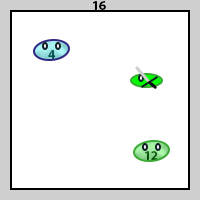
\includegraphics[width=0.45\textwidth]{Zelda-Skizze}
	\caption{Skizze der Legend of Zelda Idee\label{fig:zelda}}
\end{figure}
\subsubsection{Murmeladdierer}
Diese Idee überträgt das Vorhaben auf ein altes Murmelspiel. Es gibt mehrere Löcher, die mit Zahlen beschriftet sind, in welche die Kugeln hinein manövriert werden müssen. Die Bewegung der Kugeln wird durch das Kippen des Spielfelds in eine bestimmte Richtung erzielt. Wie in jedem der vorgestellten Ansätze wird hier eine gesuchte Zahl bereitgestellt. Da zwei Kugeln gleichzeitig auf dem Feld zu bewegen sehr schwer sein könnte, kann man das ganze auch sequenziell mit jeweils einer Kugel spielen.
\begin{figure}[htb]
	\centering
	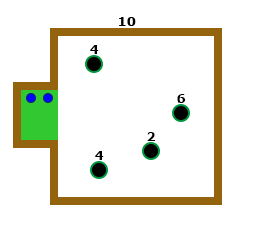
\includegraphics[width=0.3\textwidth]{HolesImg}
	\caption{Skizze des Murmeladdierer Spiels\label{fig:murmadd}}
\end{figure}
\subsubsection{Zahlenbausteine}
Auch für diese Idee ist es wieder nötig Zahlen zu einer gesuchten Zahl zu addieren. Hier sind die Zahlen in Form von Ziegelsteinen gegeben und der Spieler muss ein Gebäude errichten, welches mehrere dieser Ziegelsteine benötigt. Diese sind mit den gesuchten Zahlen beschriftet. Der Spieler muss sich zwei Steine auf dem Spielfeld suchen und diese aufeinander legen um sie zum gesuchten Ziegelstein zu addieren. Dieser muss anschließend vom Spieler an die richtige Position im Bauwerk gebracht werden.
\begin{figure}[htb]
	\centering
	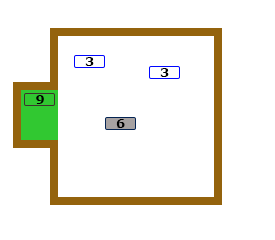
\includegraphics[width=0.4\textwidth]{BaukloetzeImg}
	\caption{Skizze des Zahlenbaustein Spiels\label{fig:baustein}}
\end{figure}
\subsubsection{MathSnake}
Für diese Idee wird das Addieren von Partnerzahlen zu einer gesuchten Zahl auf Snake übertragen. In diesem Snake gibt es Zahlenäpfel. Frisst die Schlange einen dieser Äpfel hat sie einen Teil der Partnerzahl gefressen und zur Addition hinzugefügt. Frisst sie den nächsten Apfel werden beide Zahlen addiert. Die Schlange wird pro Apfel länger und schneller.
\begin{figure}[htb]
	\centering
	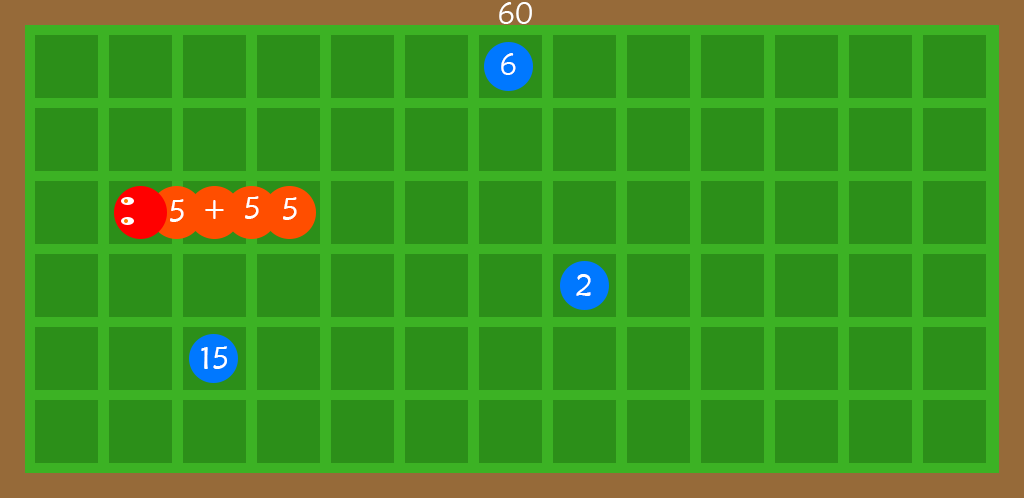
\includegraphics[width=0.49\textwidth]{Snake-Skizze}
	\caption{Skizze des MathSnake Spiels\label{fig:mathsnake}}
\end{figure}
\section{Wahl des Spielkonzepts und Entwicklung des Spiels}
Aus den erarbeiteten Konzepten habe ich mich für MathSnake entschieden, da diese Idee einem klassischen Spiel einen neuen Reiz verleiht. Die Kombination mit \textit{The Legend of Zelda} würde dies ebenfalls erfüllen, allerdings würde eine Umsetzung hier erheblich mehr Zeit in Anspruch nehmen, welche dann für die Evaluation gefehlt hätte. Außerdem bietet die MathSnake Variante mehr Möglichkeiten, das Spiel herausfordernder zu gestalten. Zum Beispiel durch Anstieg der Bewegungsgeschwindigkeit nach dem Essen eines Apfels und die Längenzunahme der Schlange. Aber auch durch weitere Features, wie dem Verfaulen der Äpfel über eine gewisse Zeit, lässt sich das Spiel schwieriger gestalten. Diese Aspekte waren ausschlaggebend um sich für die Snake Variante zu entscheiden.
MathSnake wurde in der Entwicklungsumgebung Unity umgesetzt, da diese sehr Einsteigerfreundlich ist und man bereits in kurzer Zeit gute Ergebnisse erzielen kann. Als Zielplatftorm wurde Android gewählt, um das Spiel auf einem bereitgestellten Tablet spielen zu können. Damit das Spiel möglichst professionell und kinderfreundlich aussieht, wurde sich für ein Asset-Pack aus dem Unity Asset Store entschiden. Durch dieses gab es bereits Grafiken für die Schlange und Gestaltungsdetails für die Umgebung. Die Umgebung selbst wurde in Blender modeliert und in Unity mit den gegebenen Details geschmückt.
\subsection{Verschiedene Spielversionen}
Im Zuge dieser Bachelorarbeit wurden zwei verschiedene Varianten umgesetzt und evaluiert. Zur Auswahl standen folgende Versionen mit deren erwarteten Vor- und Nachteilen.\\
\\
Dabei handelt es sich bei der TopDown-Perspektive um die Ansicht aus der Vogelperspektive auf das Spielgeschehen. Das heißt von oben mit Blick senkrecht nach unten. Während bei der Third-Person-Perspektive die Kamera direkt hinter dem Schlangenkopf positioniert wird. Die Unterschiede lassen sich in Abbildung \ref{fig:mathsnake-perspektives} erkennen.

\subsubsection{3D Snake mit Third-Person-Perspektive}
\begin{table}[h!]
\centering
\begin{tabular}{|l|l|}
\hline
\multicolumn{1}{|c|}{\textbf{Vorteile}}                                                                         & \multicolumn{1}{c|}{\textbf{Nachteile}}                                                                               \\ \hline
modern                                                                                                        & \begin{tabular}[c]{@{}l@{}}wenig Übersicht über das Spielfeld, welche Zahlen wo\\ liegen ist nicht gegeben\end{tabular} \\ \hline
\begin{tabular}[c]{@{}l@{}}mehr das Gefühl als Spieler\\ die Schlange zu sein.\end{tabular}                     &                                                                                                                       \\ \hline
\begin{tabular}[c]{@{}l@{}}Spielfeld kann abwechslungsreich\\ über mehrere Ebenen gestaltet werden\end{tabular} &                                                                                                                 \\ \hline
\begin{tabular}[c]{@{}l@{}}Übersicht auf welcher Ebene man sich\\ befindet ist sehr gut\end{tabular}            &  \\ \hline
\begin{tabular}[c]{@{}l@{}}wenig Übersicht kommt dem Such-\\ charakter allerdings zugute.\end{tabular}          &  \\ \hline
\end{tabular}
\caption{Gegenüberstellung von Vor- und Nachteilen der Variante 3D Snake mit Third-Person-Perspektive\label{fig:3dthird}}
\end{table}
\subsubsection{3D Snake mit TopDown-Perspektive}
\begin{table}[h!]
\centering
\begin{tabular}{|l|l|}
\hline
\multicolumn{1}{|c|}{\textbf{Vorteile}} & \multicolumn{1}{c|}{\textbf{Nachteile}}                                                                 \\ \hline
modern                                  & \begin{tabular}[c]{@{}l@{}}Schlechte Übersicht darüber, auf welcher\\ Ebene man sich bewegt\end{tabular} \\ \hline
mehrere Spielfeldebenen möglich         &                                                                                                         \\ \hline
Gute Übersicht wo welche Zahl liegt     &                                                                                                         \\ \hline
                                        &                                                                                                         \\ \hline
                                        &                                                                                                         \\ \hline
\end{tabular}
\caption{Gegenüberstellung von Vor- und Nachteilen der Variante 3D Snake mit TopDown-Perspektive\label{fig:3dTop}}
\end{table}
\subsubsection{2D Snake mit TopDown-Perspektive}
\begin{table}[h!]
\centering
\begin{tabular}{|l|l|}
\hline
\multicolumn{1}{|c|}{\textbf{Vorteile}} & \multicolumn{1}{c|}{\textbf{Nachteile}}                                                                         \\ \hline
einfache Umsetzung                      & kein neuer Anreiz gegenüber dem klassischen Snake                                                                                                    \\ \hline
Grafisch nicht so aufwändig             & \begin{tabular}[c]{@{}l@{}}weniger Möglichkeiten den Spieler\\ über Level-Elemente herauszufordern\end{tabular} \\ \hline
Gute Übersicht wo welche Zahl liegt     &                                                                                                                 \\ \hline
                                        &                                                                                                                 \\ \hline
                                        &                                                                                                                 \\ \hline
\end{tabular}
\caption{Gegenüberstellung von Vor- und Nachteilen der Variante 2D Snake mit TopDown-Perspektive\label{fig:2dTop}}
\end{table}
\subsection{Grid-Spielfeld}
Weiterhin stand zur Auswahl ob das SnakeSpiel mit oder ohne einem Grid-Spielfeld erstellt werden soll. Unter einem Grid-Spielfeld wird ein Spielfeld verstanden, dass in einzelne kleinere Felder aufgeteilt ist, auf denen sich die Schlange bewegen kann. Pro 'Zug' bewegt sich die Schlange jeweils ein Feld weiter und füllt dieses Feld komplett aus.
\subsubsection{Snake mit Grid}
\begin{table}[h!]
\centering
\begin{tabular}{|l|l|}
\hline
\multicolumn{1}{|c|}{\textbf{Vorteile}}                                                     & \multicolumn{1}{c|}{\textbf{Nachteile}}                                                      \\ \hline
einfache Steuerung                                                                          & \begin{tabular}[c]{@{}l@{}}weniger Freiheiten für den Spieler\\ sich zu bewegen\end{tabular} \\ \hline
\begin{tabular}[c]{@{}l@{}}einfach um neue Objekte in die\\ Spielwelt zu legen\end{tabular} & weniger Freiheiten im Leveldesign                                                            \\ \hline
\begin{tabular}[c]{@{}l@{}}Objekte können nicht ineinander\\ liegen\end{tabular}            &                                                                                              \\ \hline
                                                                                            &                                                                                              \\ \hline
                                                                                            &                                                                                              \\ \hline
\end{tabular}
\caption{Gegenüberstellung von Vor- und Nachteilen des Snake-Spiels mit einem Grid-Spielfeld\label{fig:grid}}
\end{table}
\subsubsection{Snake ohne Grid}
\begin{table}[h!]
\centering
\begin{tabular}{|l|l|}
\hline
\multicolumn{1}{|c|}{\textbf{Vorteile}}                                                                 & \multicolumn{1}{c|}{\textbf{Nachteile}} \\ \hline
moderne Steuerung                                                                                       & Objekte können ineinander liegen        \\ \hline
\begin{tabular}[c]{@{}l@{}}Spieler kann sich in mehr als\\ vier Richtungen bewegen\end{tabular}            & Aufwändiger in der Umsetzung            \\ \hline
\begin{tabular}[c]{@{}l@{}}Leveldesign kann durch verschiedene\\ Formen unterstützt werden\end{tabular} &                                         \\ \hline
                                                                                                        &                                         \\ \hline
                                                                                                        &                                         \\ \hline
\end{tabular}
\caption{Gegenüberstellung von Vor- und Nachteilen des Snake-Spiels ohne einem Grid-Spielfeld\label{fig:nogrid}}
\end{table}
Entschieden wurde sich für die beiden 3D Varianten ohne Grid, da das Ziel ist, beide Versionen vergleichen zu können um zu ermitteln, welche Version bei Spielern besser ankommt. Ein großer Vorteil, die beiden 3D Varianten zu implementieren, ist auch, dass so nur die Perspektive geändert werden kann ohne die Grafiken neu anpassen zu müssen. So blieb der Fokus auf der unterschiedlichen Perspektive auf das Spielgeschehen. Um eine moderne Steuerung zu ermöglichen, habe ich mich außerdem gegen ein Spielfeld mit Grid entschieden. 
\section{Aufbau und Funktionsweise des Spiels}
\subsection{Aufbau des Spiels}
\subsubsection{Menüführung}
Der Aufbau des Spiels ist einfach gehalten. Der Spieler beginnt das Spiel im Hauptmenü, welches in Abbildung \ref{fig:mathsnake-menu}, in Form eines Ablaufplans, dargestellt wird. In diesem kann er sich für eine Spielversion entscheiden, die Highscore Tabelle begutachten oder das Spiel beenden. Startet er eine der beiden Spielversionen beginnt direkt das Spiel. 
\begin{figure}[htb]
	\centering
	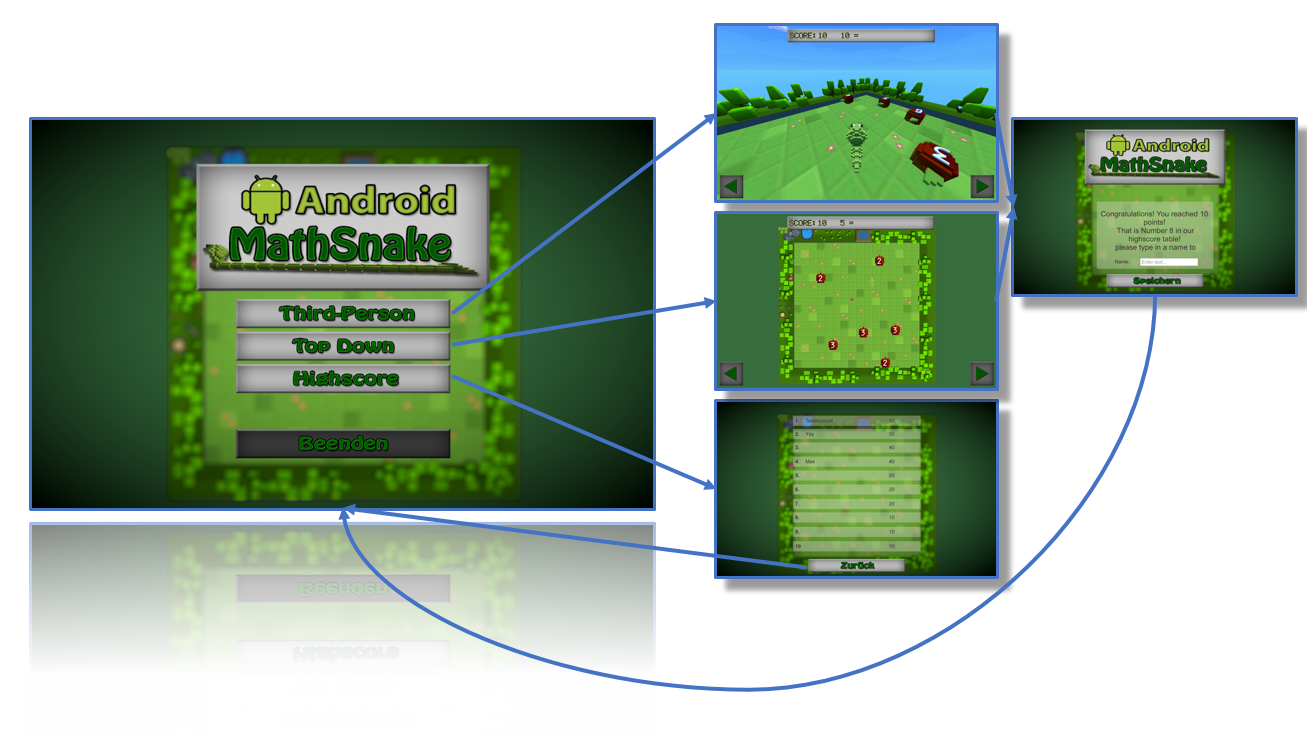
\includegraphics[width=0.85\textwidth]{MathSnake-Overview}
	\caption{Hauptmenü von MathSnake\label{fig:mathsnake-menu}}
\end{figure}
\subsubsection{Spielfeldaufbau}
Der Spieler sieht am oberen Bildschirmrand die gesuchte Zahl gefolgt von einem '=' ( Beispielsweise ' 5 = ' ). Auf dieses folgen dann alle gefressenen Zahlen mit einem '+' verbunden ( z.B. 5 = 1 + 1 + 3 ). Dies stellt die Gleichung dar, die erfüllt sein muss, um die Aufgabe zu bestehen. Links neben der gesuchten Zahl findet der Spieler auch seinen aktuellen Score. Dieser nimmt bei einer falschen Zahl ab und bei einer richtigen Zahl zu. Der Spieler kann die Schlange über zwei Pfeiltasten steuern. Diese zwei Tasten geben die Richtung an, in die sich die Schlange bewegen soll. Der Spieler kann sie über diese Tasten nach rechts oder links bewegen. Die einzelnen Felder werden auch nochmals in der Abbildung \ref{fig:mathsnake-setup} verdeutlicht.
\begin{figure}[htb]
	\centering
	\includegraphics[width=0.75\textwidth]{MathSnake-setup}
	\caption{Ansicht auf den Aufbau des Spiels\label{fig:mathsnake-setup}}
\end{figure}
\subsubsection{Highscore}
Das Spiel stellt auch eine simple Highscore Liste bereit, um einen weiteren Anreiz zu schaffen. Diese wird für den Nutzertest deaktiviert, da die Nutzer sich voll auf die Bewertung des Spiels an sich konzentrieren sollen und der Highscore nicht Teil der Forschungsfragen ist.\\
Ist der Highscore aktiviert, wird dem Spieler nach dem Ende einer Spielrunde eine Nachricht angezeigt. Dem Spieler wird in dieser angezeigt, ob er genügend Punkte gesammelt hat, um sich in der Highscore Liste einzutragen. Dies geschieht dann über ein Textfeld in dessen er seinen Name eingeben kann, wie in Abbildung \ref{fig:mathsnake-newHighscore} zu sehen ist.
\begin{figure}[htb]
	\centering
	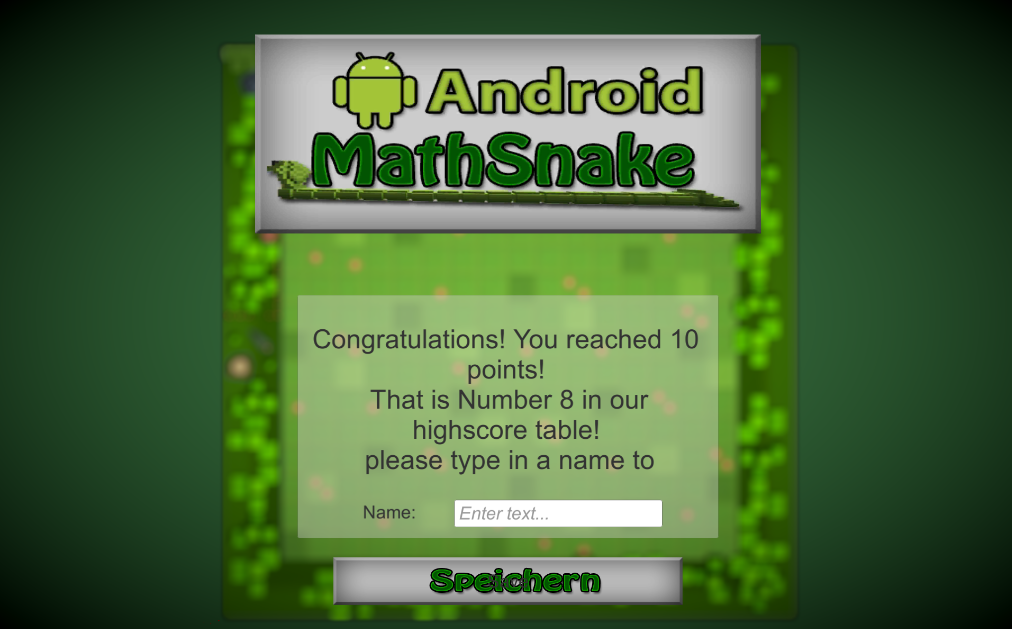
\includegraphics[width=0.65\textwidth]{MathSnake-Highscore1}
	\caption{Erstellen eines neuen Highscore-Eintrags\label{fig:mathsnake-newHighscore}}
\end{figure}
Im Hauptmenü kann, wie in Abbildung \ref{fig:mathsnake-menu} zu erkennen ist, die aktuelle Highscore-Tabelle angezeigt werden. Diese ist so aufgebaut, dass Platz 1 mit der höchsten Punktzahl oben steht. Gibt es Spieler mit der gleichen Punktzahl schlägt ein neueres Ergebnis ein Älteres. In Abbildung \ref{fig:mathsnake-HighscoreTable} ist eine beispielhafte Ansicht der Highscore-Tabelle abgebildet.
\begin{figure}[htb]
	\centering
	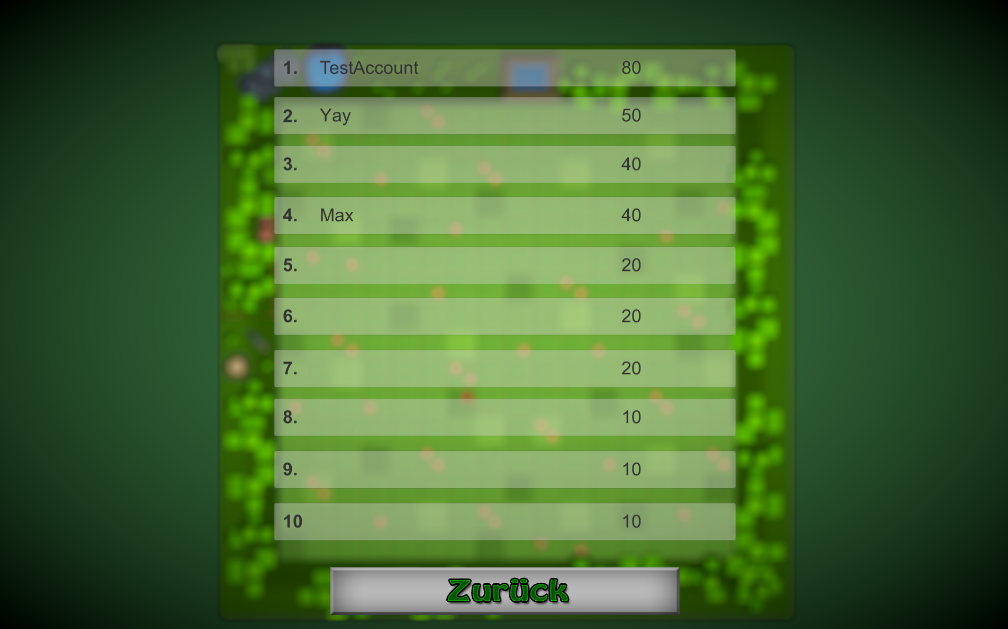
\includegraphics[width=0.65\textwidth]{MathSnake-Highscore2}
	\caption{Ansicht der Highscore-Tabelle\label{fig:mathsnake-HighscoreTable}}
\end{figure}
\subsection{Funktionsweise des Spiels}
Das entwickelte Spiel lässt sich nun entweder in der TopDown Ansicht oder in der Third-Person Ansicht spielen. Die Funktionsweise bleibt bei beiden identisch. Der Spieler steuert eine Schlange und kann diese mit zwei Pfeiltasten nach rechts oder links drehen, um die Bewegungsrichtung zu verändern. Am oberen Bildschirmrand wird ihm eine gesuchte Zahl, sowie seine aktuelle Punktzahl, angezeigt. Hat die Schlange einen Apfel mit einer Zahl gefressen wird diese durch ein + getrennt dem Gleichtungsbereich(siehe \ref{fig:mathsnake-setup}) hinzugefügt. Mit jedem gegessenem Apfel wird die Schlange schneller und länger.
\begin{figure}[htb]
	\centering
	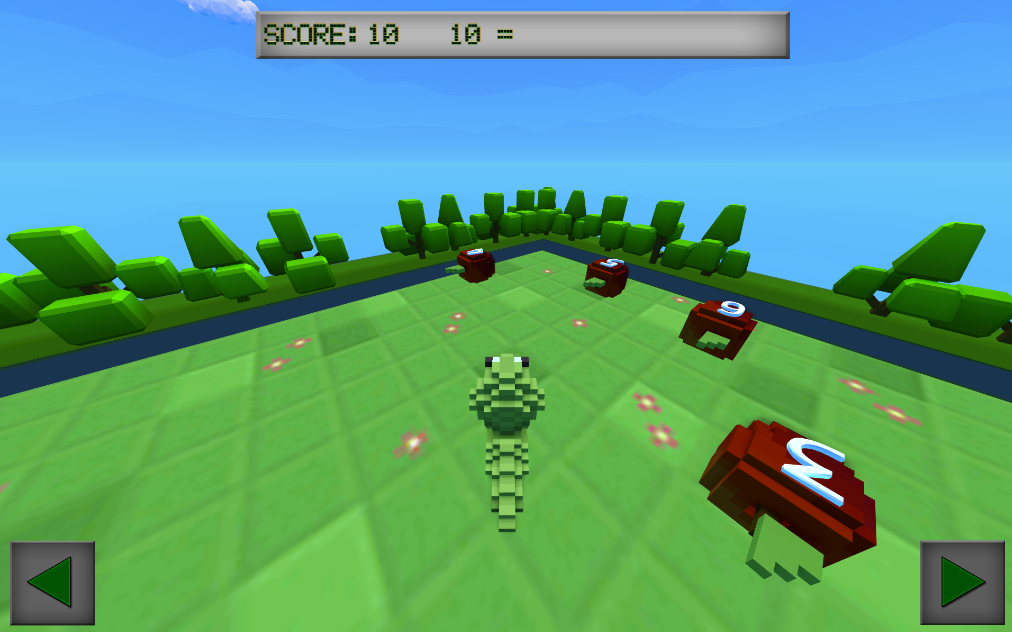
\includegraphics[width=0.35\textwidth]{MathSnake-ThirdPerson}
	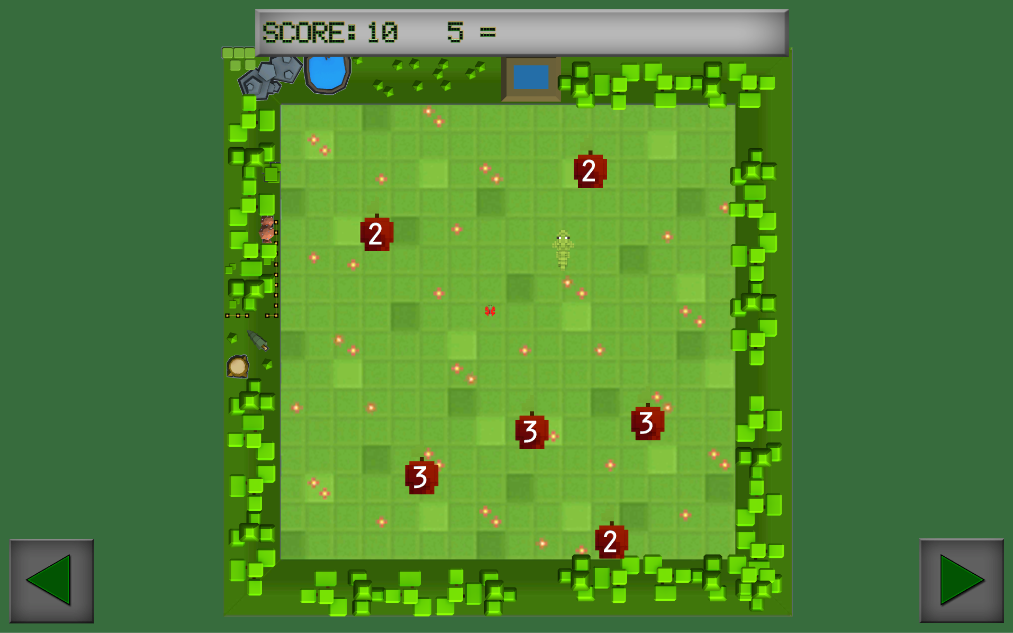
\includegraphics[width=0.35\textwidth]{MathSnake-TopDown}
	\caption{Links: Third-Person und Rechts: TopDown Perspektive\label{fig:mathsnake-perspektives}}
\end{figure}
\subsubsection{Levelsystem}
Pro zu suchender Zahl gibt es ein Level. Um das Spiel auf Dauer herausfordernder zu gestalten, wurde ein kleines Levelsystem eingeführt. Dabei varriiert der Zahlenraum je nachdem in welchem Levelbereich der Spieler sich befindet. Im höchsten Bereich beginnen die Äpfel zu verfaulen. Die implementierte Zuordnung ist der Tabelle \ref{tab:levels} zu entnehmen.
\begin{table}[h!]
\centering
\begin{tabular}{|l|l|l|}
\hline
\textbf{Level} & \textbf{Zahlenbereich} & \textbf{Eigenschaften}       \\ \hline
0-4            & 3-20                   & -                            \\ \hline
5-9            & 20-50                  & -                            \\ \hline
10-19          & 50-100                 & -                            \\ \hline
20-49          & 30-100                 & -                            \\ \hline
50+            & 30-100                 & Äpfel verfaulen mit der Zeit \\ \hline
\end{tabular}
\caption{Bedeutung der einzelnen Levelbereiche\label{tab:levels}}
\end{table}
